%*******************************************************************************
%****************************** Second Chapter *********************************
%*******************************************************************************

\chapter{Dereverberation using NMF}

In the time domain, reverberation is modeled simply as the convolution between the source signal and the room impulse response. 
\begin{align}
y(t) = s(t)*h(t) \label{eq :1}
\end{align}
Here, $s(t)$ is the original speech signal, $h(t)$ is the impulse response of the room, henceforth mentioned as the RIR(Room Impulse Response) and $y(t)$ is the observed speech signal. It is assumed that the room impulse response $h(t)$ does not change with time. This implies that the system modeled is a linear time-invariant (LTI) system. In the time domain, inverse filtering techniques have been developed to recover clean speech from reverberant speech through application of an adequate adaptive filter. The objective is to calculate $h(t)$, the room impulse response and apply its inverse filter to $y(t)$ to obtain $s(t)$. One major issue with time domain filtering is its lack of robustness against speaker movements, which cause a change in the phase of the signal, changing the RIR, i.e. $h(t)$. 
This is why, we have chosen the magnitude spectrogram domain to model and remove reverberant effects from speech. That is, given a spectrogram corresponding to a speechs signal which is recorded in a reverberant environment, the objective will be to counter the effects of reverberation and estimate the magnitude of the clean speech signal. As discussed in Chapter 1, there is an evident smearing effect in the spectral feature domain because of reverberation. This is exactly the intuition for the class of techniques that are discussed henceforth.




 \section{Non negative matrix factor deconvolution (NMFD)}
Consider a signal $y(t)$ which is a recorded version of a source signal $s(t)$ in a reverberant environment.  $Y$ is the magnitude spectrogram, obtained by taking the short time fourier transform (STFT) of $y(t)$. Given $Y$, the task is to estimate $X$, which is the magnitude spectrogram of the clean speech signal. A basic model for the relating these two magnitude spectrograms is \cite{naka} \cite{moham}-
\begin{align} Y_k[n] \approx Y_k[n]' = \sum_{\tau = 0}^{\tau = L-1} X_k[n - \tau] * H_k[\tau] \label{convolution}
 \end{align}
 

Here, $Y_k$ is the $kth$ frequency sub-band of $Y$, similarly, $X_k$ is the $kth$ frequency sub-band of $X$ and $H_k$ is a sub-band filter, of length $L$ which models the smearing of the clean spectrum sub-band. It is $H_k$ and $X_k$ that have to be estimated from the given $Y_k$, under reasonable constraints. Although in much of the literature, $H$, is said to be the STFT of the room impulse response $h[n]$, there is little evidence in literature that it has any obvious relation to the actual room impulse response . For now though, it will be called the RIR and its relationship with the actual room impulse response will be discussed later. $\hat{Y}$, which is the approximation of the magnitude spectrogram of reverberant speech, $Y$, can have an infinite number of decompositions, $X$ and $H$ which satisfy the above equation. Not all of the solutions though, will give us an estimate of the clean speech magnitude spectrogram and the RIR respectively. Thus, constraints have to be used to narrow the solutions to get more meaningful results. More specifically, we need to ensure that $X$ resembles a speech spectrogram and $H$, a room impulse response spectrogram. 

It has been established that speech magnitude spectrograms are sparse across speakers and utterances. This property has been used in \cite{naka} \cite{moham}\cite{gamma} to arrive at a cost function that gives a quantitative measure of the distance from a desirable solution. The cost function is defined as- 
\begin{align} f(X,H) = \sum_{k,t} (Y_k[t] - Y'_k[t])^2 + 2 \lambda \sum_{k,t} |X_k[t]| \label{cost}
\end{align}
The first term signifies the squared sum of the distances of the coefficients of $Y$ and $Y'$ and the second term enforces sparsity of the clean speech spectrogram.Fpr the underlying assumptions and derivation for this cost function, see \cite{naka}. Clearly, a closed-form solution to the above equation is not possible for (3.3) This problem that is similar to the problem of Non-negative Matrix Decomposition(NMF) discussed in Chapter 2, where a similar cost function was used. To minimize the cost function, we used the gradient descent algorithm to arrive at iterative multiplicative updates which converged to a solution. Similarly, for the cost function in (3.3), multiplicative updates can be derived for $X$ and $H$ as well. With the sparsity constraint on $X$, the iterative multiplicatssive updates for the dereverberation problem are given in \cite{naka} as 
\begin{align}X_k[\tau] = \hat{X}_k[\tau]\frac{\sum_{t}\hat{H_k}[t-\tau]Y_k[t]}{\sum_{t}\hat{H_k}[t-\tau]\hat{Y'_k}[t] + \lambda} \label{X update}
\end{align}
\begin{align} H_k[\tau] = \hat{H}_k[\tau]\frac{\sum_{t}\hat{X_k}[t-\tau]Y_k[t]}{\sum_{t}\hat{X_k}[t-\tau]\hat{Y'_k}[t]} \label{H update}
\end{align}
Here, $\hat{H}$, $\hat{Y}$ and $\hat{X}$ are the estimates from the previous iteration. These updates are based on the gradient descent algorithm that converges to a local minimum. No specific property for H is exploited, to avoid scale ambiguity, the sum of the coefficients of each sub-band is scaled down to sum to one i.e. $\sum_{t}H_k[t] = 1 \ \ \forall k$. This constraint is not imposed in the updates. Rather after each iteration, each row of H is normalized to account for this constraint. For speech, the only property that has been used to enforce a constraint on $X$, is its sparsity in the magnitude spectrogram domain. In the next few sections, we modify the above approach to incorporate specific properties.

\section{Activation Deconvolution}
The technique of non-negative matrix factorization efficiently separates the temporal and the spectral features of the magnitude spectrogram of the speech signals in the activation matrix and the basis vectors respectively. Reverberation can be modeled as a largely temporal phenomenon where delayed and attenuated versions of the signal corrupt the recorded signal. Our hypothesis is that since reverberation is a temporal phenomenon, its effects will be localized to the temporal part of the non-negative factors, which is the activation matrix

Figures \ref{activations_clean} and \ref{activation_reverb} are the activation patterns for two speech signals.Figure \ref{activations_clean} shows the activation pattern that was obtained by applying NMF on a sentence recording from the TIMIT database. Figure \ref{activation_reverb} on the other hand shows activation patterns for the same audio signal, with reverberation added. There is a strong correlation between the activation patterns. We hypothesis that an activation vector for the clean speech spectrogram, $A_i$, corresponding to a basis vector $i$ undergoes the following transformation when reverberation is added to  the clean speech signal.
\begin{align}
A_i^{reverb}(t) = A_i(t)*h(\tau)
\end{align}
Therefore, given the reverberant signal, we can obtain the activation vectors $A_{i}^{reverb}$ . Then using the Non-Negative factor deconvolution technique, presented in the previous section, $A_i$ can be isolated. Notice how this equation is similar to Equation \ref{convolution}. Thus, we use the same updates in Equations \ref{X update} and \ref{H update} to estimate the clean speech activation vector $A_i(t)$ from the reverberant activation vectors $A_i^{reverb}$. A spectrogram is then reconstructed using these activations. Figure \ref{input_spec} shows the spectrogram of a speech signal from the TIMIT database with added reverberation. Figure \ref{filtered spec} shows the spectrogram obtained after the activations were processed using the above mentioned algorithm. It can be clearly seen that the smearing of the spectrogram has been visibly reduced. 

\begin{figure}
\centering
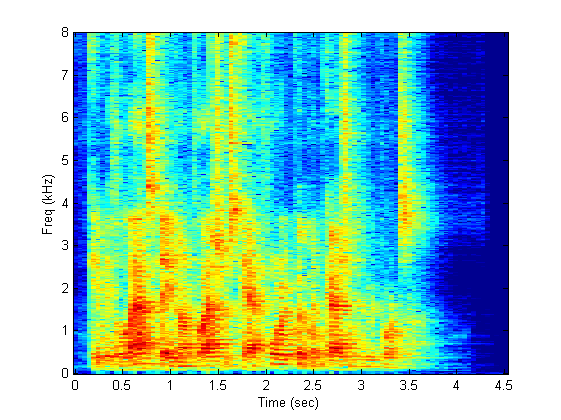
\includegraphics[scale=0.6]{input_spectrogram}
\caption{ Spectrogram for a reverberated speech signal. Key parameters - Sampling frequency : $16000kHz$. Window : hanning window of length 1024 samples. Overlap : 512 samples. Size of fft: 1024 } \label{input_spec}
\end{figure}

\begin{figure}
\centering
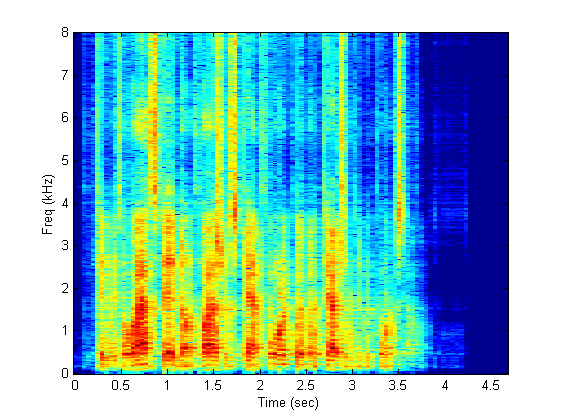
\includegraphics[scale=0.6]{filtered_activation_spectrogram}
\caption{Spectrogram after the activations were processed. Notice the reduction of the spectrogram smearing from Figure \ref{input_spec} . Key parameters - Sampling frequency : $16000kHz$. Window : hanning window of length 1024 samples. Overlap : 512 samples. Size of fft: 1024 } \label{filtered spec}
\end{figure}

\begin{figure}
\centering
\begin{minipage}{.5\textwidth}
  \centering
  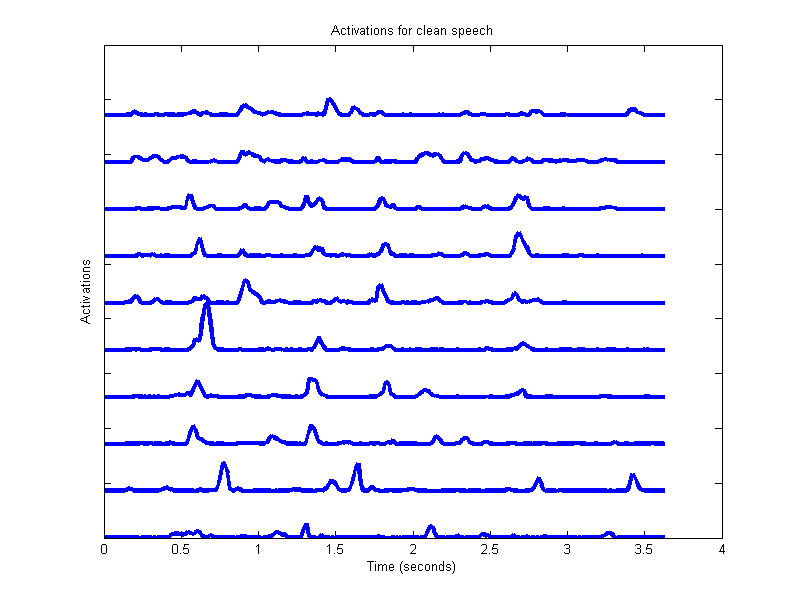
\includegraphics[width=.9\linewidth]{activations_clean}
  \captionof{figure}{Activations in clean speech} \label{activations_clean}
  \label{fig:test1}
\end{minipage}%
\begin{minipage}{.5\textwidth}
  \centering
  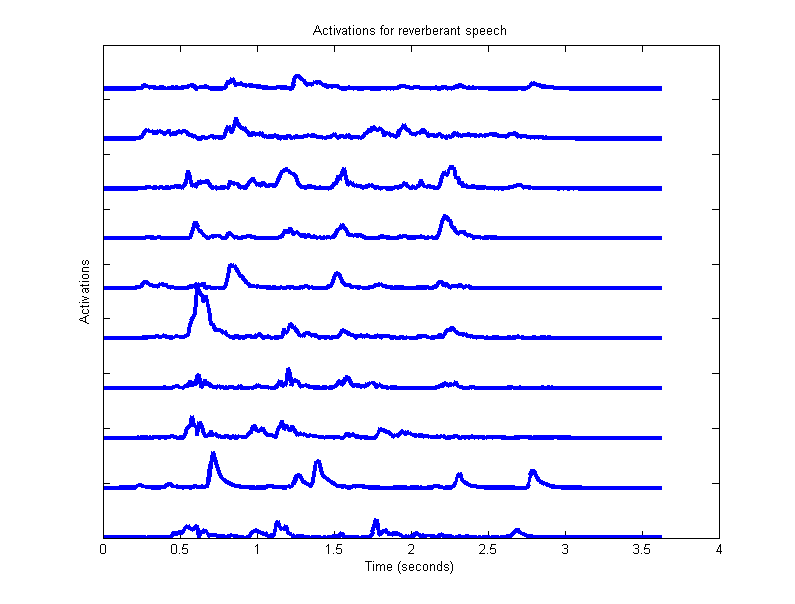
\includegraphics[width=.9\linewidth]{activations_reverb}
  \captionof{figure}{Activations in reverberant environment} \label{activation_reverb}
  \label{fig:test2}
\end{minipage}

\end{figure}
\section{NMFD using NMF model for speech}
The imposition of constraints in NMFD ensures that the solution converges to a clean speech spectrogram. A better model for speech or RIR($X$ and $H$ respectively) will ensure convergence to a better solution. In section 3.1, we have only exploited that speech is sparse in the magnitude spectrogram domain. NMF has been shown to be an efficient way to represent speech by decomposing it into factors with significantly less dimensions. It is based on the assumption that speech spectrograms are low rank. NMF tries to find an encapsulating basis vector set to represent the whole spectrogram.  This representation has been shown to work in separation  \cite{paris} and dereverberation \cite{baby} very well. We now incorporate this representation into the Non-Negative factor deconvolution model discussed in the previous section as suggested in \cite{moham}.

Given input magnitude spectrogram, $Y$, of a time domain reverberated signal, $y(t)$ we can use NMF to decompose into a basis matrix $W$ and an activation matrix $X$ such that $ S = W*X$ and $Y \approx S$. 
Now, we will introduce a cost function, as given in \cite{moham}, which quantifies the distance of the current estimate from the desired solution. This cost function is based on the Kullback-Leiber(KL) divergence, which has been shown to be better suited to speech applications than the sum squared error used in \cite{naka}. The cost function using KL divergence, without including the NMF representation for speech is given by -
\begin{align}
f(Y,S,H) = \sum_{k,t} KL( Y(k,t) \ | \ \sum_{\tau = 0}^{L}H(k, \tau)S(k,t-\tau) ) + \lambda \sum_{k,t}S(k,t)
\end{align}

$L$ is the length of the RIR in the spectrogram domain. $\lambda$ is the sparsity parameter. Now, NMF models $S$ as a combination of two matrices, $W$ and $X$. The modified cost function, incorporating this relationship is -
\begin{align}
f(Y,W,X,H) = \sum_{k,t} KL(Y(k,t)|\sum_{\tau = 0}^{L}H(k, \tau)\sum_{r =1}^{R}W(k,r)X(r,t-\tau)) + \lambda \sum_{r,t}X(r,t)
\end{align}
For this modified cost function, the multiplicative updates for the gradient descent algorithm are given in \cite{moham}.
\begin{align}H(k,\tau) = \hat{H}(k,\tau) \frac{\sum_{t}Y(k,t)\hat{S}(k,t - \tau)/\hat{Y'}(k,t)}{\sum_{t}\hat{S}(k,t - \tau)}
\end{align}

\begin{align}W(k,r) = \hat{W}(k,r) \frac{\sum_{t,\tau}Y(k,t)H(k,\tau)\hat{X}(r,t - \tau)/\hat{Y'}(k,t)}{\sum_{t,\tau}H(k,\tau)\hat{X}(r,t - \tau)}
\end{align}
\begin{align}X(r,t) = \hat{X}(r,t)\frac{\sum_{t,\tau}Y(k,t + \tau)H(k,\tau)W(k,r)/\hat{Y'}(k,t + \tau)}{\sum_{k,\tau}H(k,\tau)W(k,r) + \lambda}
\end{align}

Here,
$Y'[k,t] = \sum_{\tau}H[k,t]*S[k,t - \tau]$  and $S = W*X$. Also, $\hat{Y'}, \hat{X},\hat{S} \ and \  \hat{H}$ correspond to the values of $Y,X,S \ and \ H$ from the previous iteration respectively. 
After an appropriate number of iterations, an estimate for the clean speech spectrogram is given as $S = W*X$. 
Including the NMF representation into the NMFD approach improves the quality of the clean speech spectrogram, $S$ \cite{moham}. This has been shown in literature and will be demonstrated experimentally in Chapter 4. In the next section, we incorporate another fundamental property of speech, namely, temporal continuity. 
\section{Exploiting temporal dependencies of speech }
In section 3.2 and 3.3, two properties of speech have been incorporated into the dereverberation model, the sparsity of magnitude spectrogramdomain and the low rank nature of the magnitude spectrogram (through NMF decomposition). Temporal continuity is another property of speech that can possibly be exploited to model the speech signal better. In this section, two techniques will be discussed which model the temporal dynamics of speech and can be implemented in a similar fashion to the previous techniques with modifications to the update rules.
\subsection{Frame stacking} 
A frame stacked approach proposed in \cite{moham} is taken to exploit the fact that the magnitude spectrograms is temporally dependent. A sliding window of length $T_{stack}$ is passed through the time axis of $Y$ and each resultant frame is stacked to form a vector of dimension $K \times T_{stack}$. These vectors are then put together to form a higher dimensional matrix, $\tilde{Y}$. Now, $\tilde{Y}$ is decomposed using NMF and the algorithm follows the same as in the previous section. $W$ will now be a $KT_{stack} \times R$ matrix. The multiplicative updates for $W$ and $X$ remain the same as in (3.10) and (3.11), and the modified updates for $H$ as given in \cite{moham} are -
\begin{align}H(k,\tau) = \hat{H}(k, \tau)\frac{\sum_{l=1}^{T_{stack}}\sum_{t}\tilde{Y}(f_l,t)S(f_l,t -\tau)/\hat{Y'}(f_l,t)}{\sum_{l=1}^{T_{stack}}\sum_{t}S(f_l,t - \tau)}
\end{align}
Here, $f_l = k + l(K-1)$ . This update is essentially taking an average over all the stacked up spectrograms for an estimate of $H$. After convergence, the clean speech magnitude spectrogram is estimated as $S=G*Y$ where G is the gain function given by -
\begin{align}
G(k,t) = \frac{\sum_{l=1}^{T_{stack}}\sum_{r}W_{final}(k_l,r)X_{final}(r,t)}{\sum_{l=1}^{T_{stack}}\sum_{t}H_{stack}(f_l,\tau)W_{final}(k_l,r)X_{final}(r,t- \tau)}
\end{align}
The subscript final denotes that the values used are after all updates have been done and the algorithm has converged. $H_{stack}$ is the RIR matrix. The results and relative performance for this technique is discussed in Chapter 4. As per our experiments, it does not improve the performance of the algorithm discussed in the previous section. In the next section, we introduce another technique through which the temporal continuity of speech can be exploited.

\subsection{Convolutive NMF}
Another way to exploit the continuous nature of speech signals is by using the convolutive Non-negative matrix factorization . This technique was discussed in Section 2.3 and is used to extend the the expressive power of the basis vectors which constitute $W$ by adding to them a temporal dimension. It has already been used in source separation and enhancement applications. \cite{baby} uses the Convolutive model for dereverberation, but relies on learning the basis offline.
To include this model for speech in the dereverberation algorithm, the modified update equations are given as - 


\begin{align}X(r,t) = \hat{X}(r,t)\frac{\sum_{\alpha = 1}^{T_{base}}\sum_{k,\tau}Y(k,t + \tau)H(k,\tau)W(k,r,\alpha)/\hat{Y'}(k,t + \tau)}{\sum_{k,\tau}H(k,\tau)W(k,r) + \lambda}
\end{align}

The update equations for $W$ and $H$ remain the same. Here, $T_{base}$ is the time length of the exemplars which comprise $W$.  These updates were adopted from \cite{baby} where they have been used to achieve dereverberation is a supervised manner. 

In this chapter, we have discussed four techniques to handle reverberation in the magnitude spectrogram domain. Non-Negative Factor deconvolution(NMFD) forms the core of all these techniques. Activation matrix deconvolution is essentially NMFD applied on the activation matrix instead of the speech spectrogram. Further, NMF representation for speech is included in the NMFD technique. Then, to exploit the temporal dependencies of speech, the frame stacked model and the convolutive NMF representation  were included. All these techniques are implemented in very similar ways. Each of them has an associated cost function which is to be minimized to get non-negative matrix factors with desirable properties. Using the updates suggested by \cite{lee}, each of these cost functions are minimized using multiplicative iterative updates.

In the next chapter the implementation details are presented and performances  of these techniques are compared based on two objective measures - Perceptual evaluation of speech quality (PESQ) and Cepstral Distortion(CD).




















